\subsection{Measure \& Sketch}
\subsubsection{Vorstellung}
Die App \ms{} von \emph{SameBits} entwickelt.
Zur Zeit des Downloads (20. Januar 2018) ist die Applikation laut Google Play-Store auf zwischen $100.000$ und $500.000$ Android-Geräten installiert.
Auch diese Applikation ist unter der Kategorie ``Effizienz'' gelistet, und wird vom Entwickler mit den folgenden Worten beschrieben \citep{BitsMS}:

\begin{quote}
  ``Die Must-Have Zeichenapp für alle echten Ingenieure, Architekten, Bauarbeiter, Immobilienmakler, Handwerker wund [sic] natürlich für alle Heimwerker!''
\end{quote}

\noindent
Beim initialen Start der App wird der Benutzer mit Hilfe eines Overlays auf die möglichen Aktionen, die er in diesem Zustand tätigen kann, hingewiesen.
Hier bietet sich die Option zwischen den bestehenden Projekten zu wechseln, oder ein Neues anzulegen.
Über den Knopf ``Neu'' (siehe \autoref{fig:msmenu} kann der Nutzer ein neues Bild aufnehmen, oder direkt eines aus der Galerie importieren. \\

\begin{figure}[h]
  \centering
  \begin{subfigure}[t]{0.4\textwidth}
    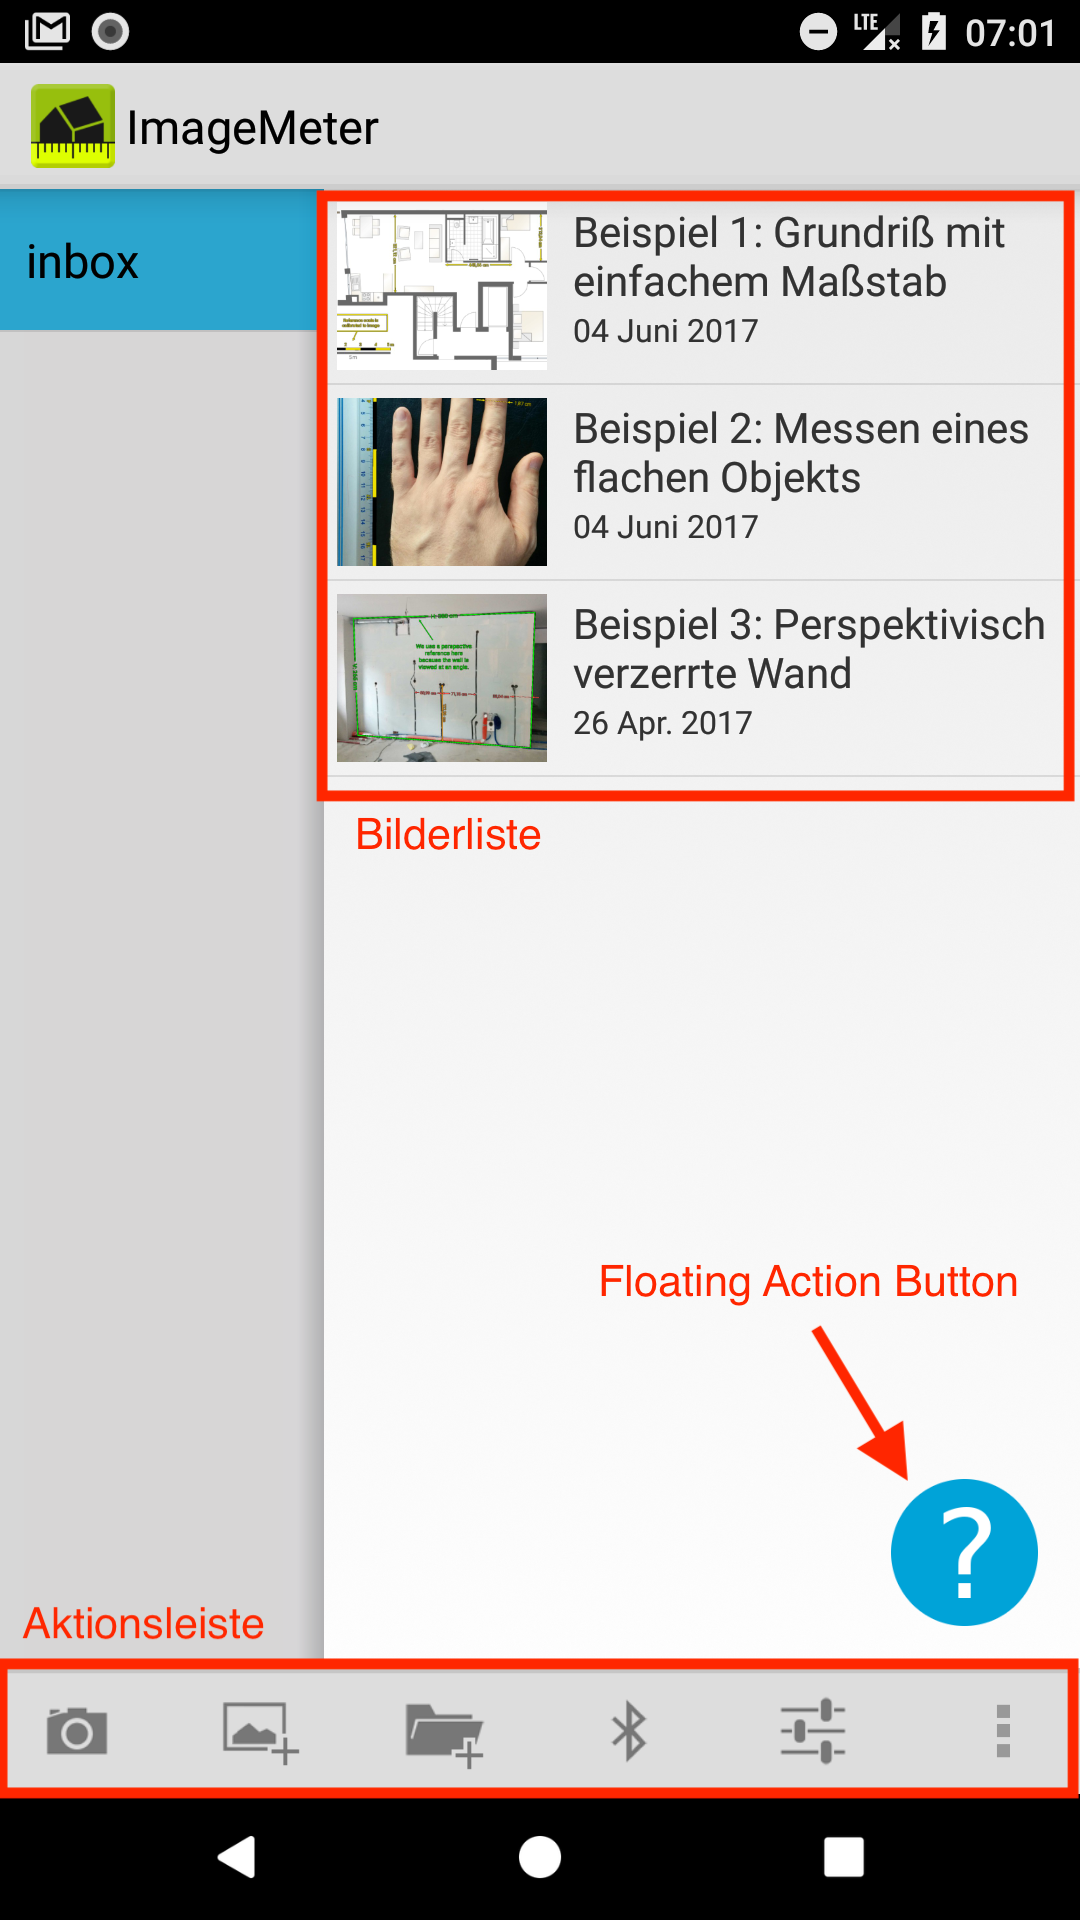
\includegraphics[keepaspectratio, width=\textwidth]{measure_sketch/menu}
    \caption{Startbildschirm}
    \label{fig:msmenu}	
  \end{subfigure}
  \begin{subfigure}[t]{0.4\textwidth}
    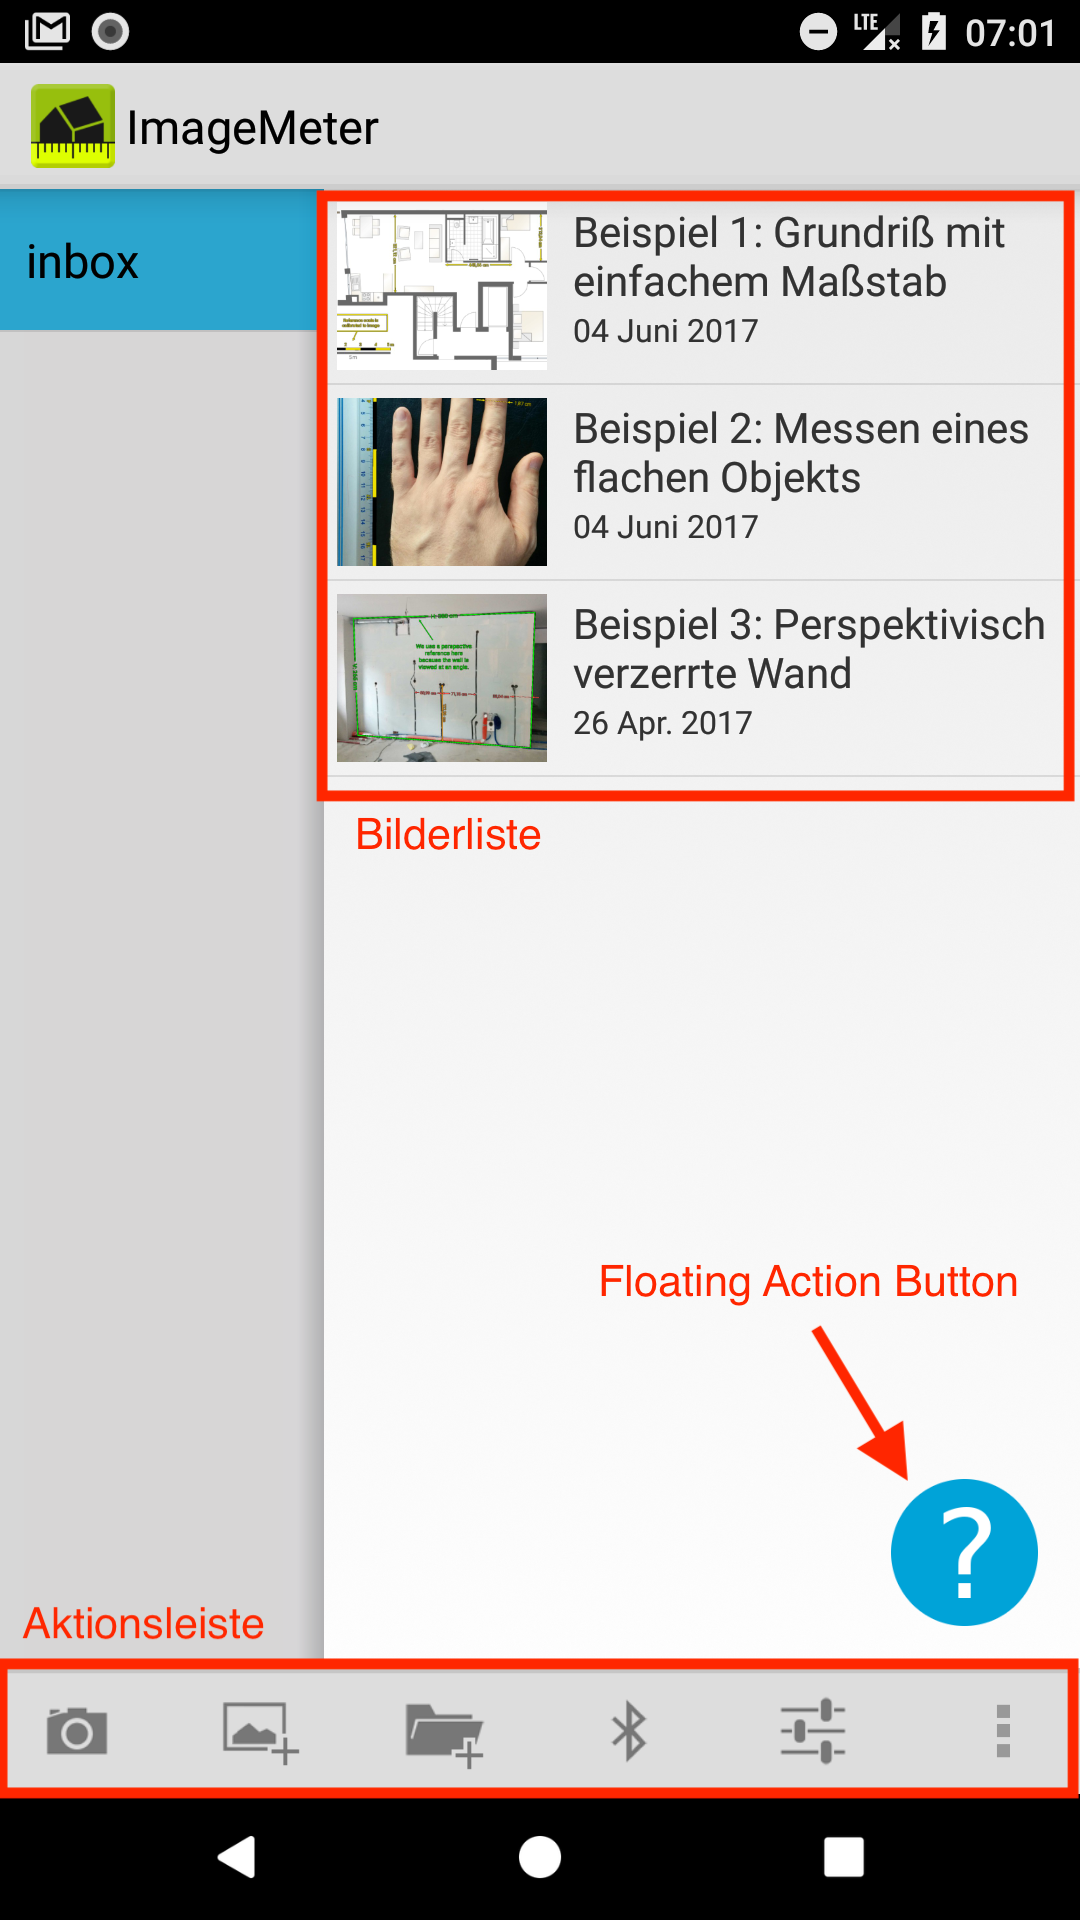
\includegraphics[keepaspectratio, width=\textwidth]{measure_sketch/menu}
    \caption{Aufmaße-Funktion} 
    \label{fig:msbar}	
  \end{subfigure}
  \caption{\ms{} beim Start der App und in der Aufmaße-Funktion}
\end{figure}

\noindent
\todo{Bilder mit Overlay}
Sobald man ein Bild ausgewählt hat, öffnet sich eine neue Benutzeröberfläche, in der, wie schon beim Start der App, durch ein Overlay alle möglichen Aktionen beschrieben werden (siehe \autoref{fig:msbar}).
In dieser Ansicht kann man das Bild mit drei verschiedenen Formen (Linie, Winkel, Freitext) annotieren. 
Zusätzlich können eingezeichnete Formen mit Messwerten beschriftet werden.\\

Weiterhin bietet sich die Gelegenheit, das bearbeitete Bild zur Galerie, \emph{Evernote} oder Universal \todo{gucken was gemeint ist} zu exportieren, oder direkt per E-Mail zu verschicken.
Auch bei dieser App kann man modifizierte Bilder speichern, und zu einem späteren Zeitpunkt zur Weiterverarbeitung wieder öffnen. \\

\subsubsection{Evaluation}

Das Hilfe-Overlay, welches beim ersten Start der App, sowie dem Öffnen der Aufmaß-Funktion angezeigt wird, zeigt dem Benutzer zwar, welche Aktionen duchführbar sind, der erklärende Text ist jedoch zu lang, sodass das Overlay viel mehr eine überfordernde, als hilfreiche Funktion hat (Nielsen~\autoref{itm:N10}).

\begin{wrapfigure}{R}{0.5\textwidth}
  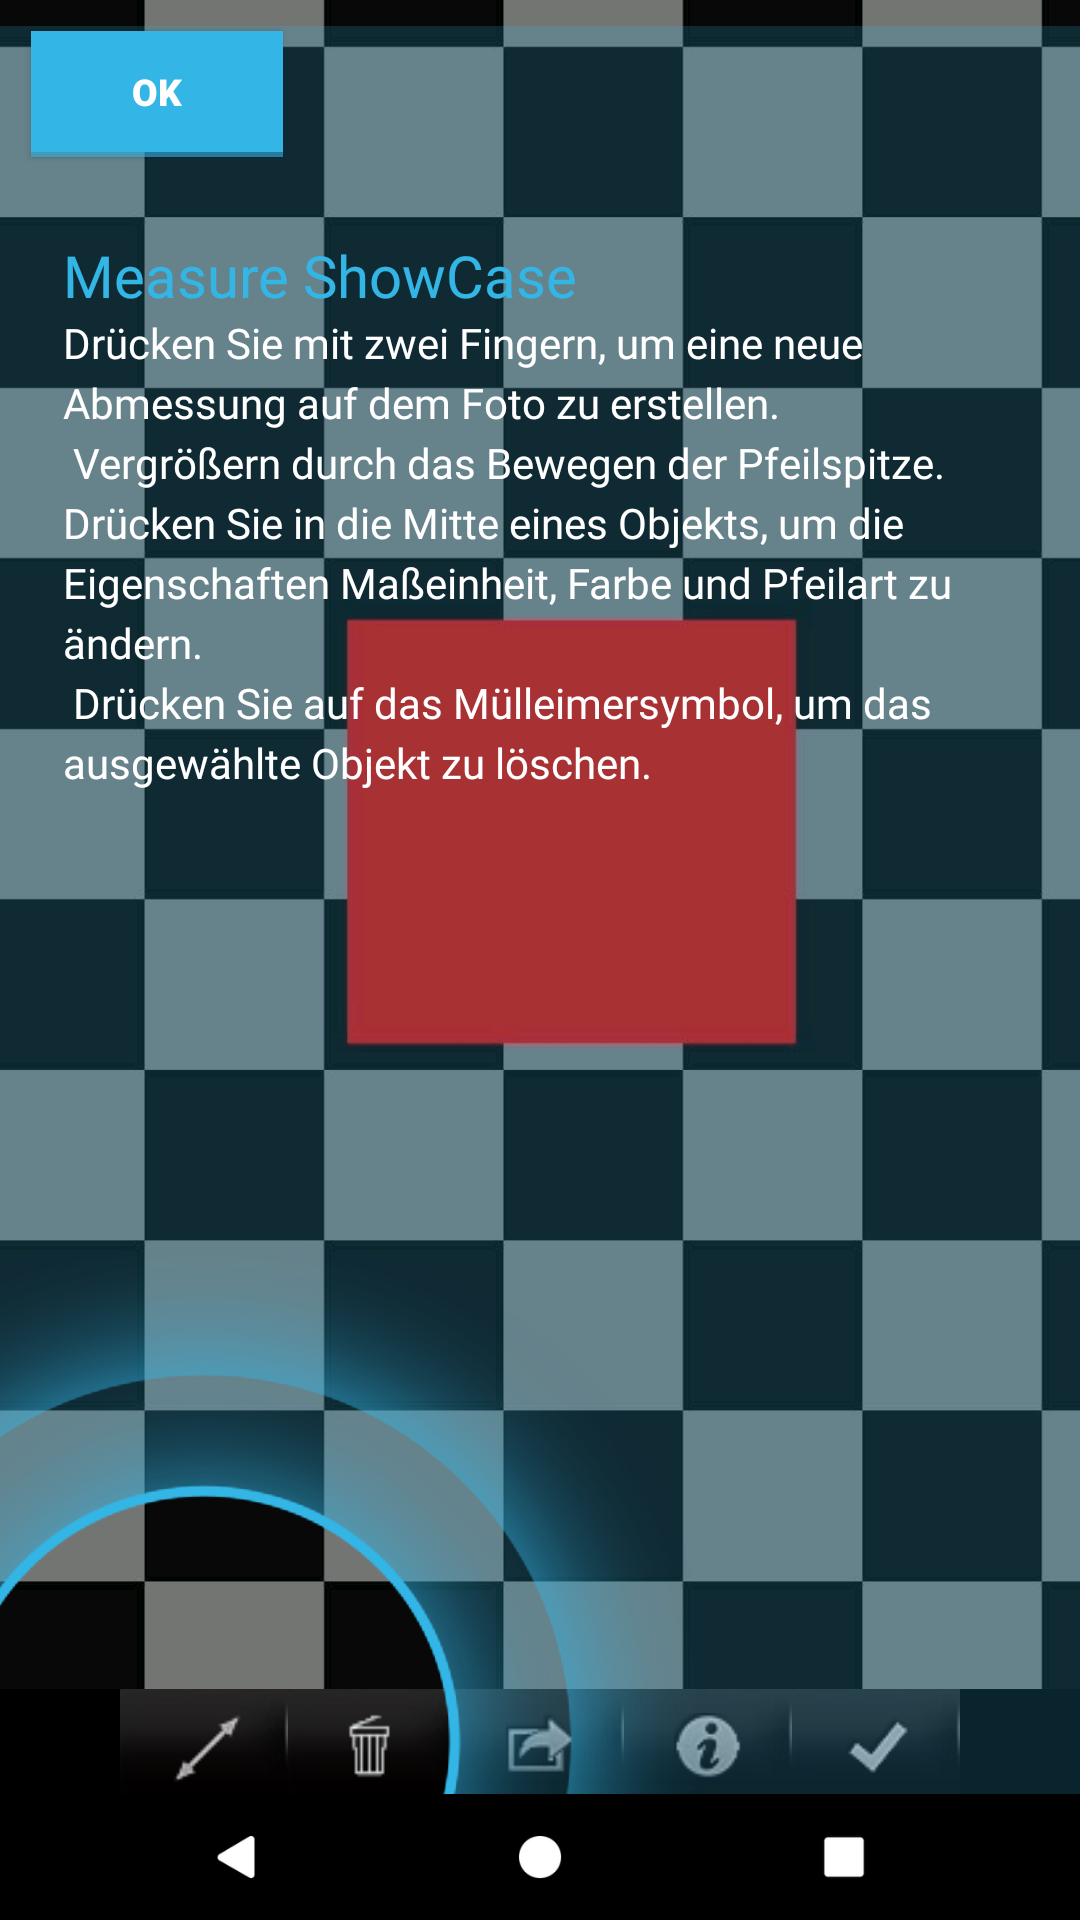
\includegraphics[keepaspectratio, width=0.5\textwidth]{measure_sketch/help_pic}
  \caption{Hilfe-Overlay beim Start der Aufmaß-Funktion}
  \label{fig:mshelp}
\end{wrapfigure}

Der aktuelle Systemzustand der App ist zwar deutlich durch die Statusleiste am unteren Bilschirmrand (siehe \autoref{fig:mshelp} erkennbar, welche Aktionen aber derzeit nicht-ausführbar ist, wird durch diese nicht ersichtlich (Nielsen~\autoref{itm:N1}). 
So werden nicht-ausfühbare Aktionen weder ausgegraut noch anders gekennzeichnet, was wiederum zur Folge hat, dass der Benutzer in ``Trial and Error''-Manier die verschiedenen Aktionen ausprobieren muss, um festzustellen, welche aktuell ausführbar sind und welche nicht (Nielsen~\autoref{itm:N5}) \\

Das Feedback zu ausgeführten Aktionen des Benutzer bleibt in den meisten Fällen aus.
Dieses fehlende Feedback gepaart mit der fehlenden Undo/Redo-Funktionalität führt zu Fehlern, die der Benutzer nur durch Wiederholung der zuvor ausgeführten Aktionen bis vor dem Fehlerzustand beheben kann (Nielsen~\autoref{itm:N3} \& \autoref{itm:N9}). \\

Einen ``Experten-Modus'', in Form von Abkürzungen für häufig ausgeführte Aktionen, gibt es nicht (Nielsen~\autoref{itm:N7}).
So muss der Nutzer beispielsweise um die Farbe der nocht einzuzeichnenden Formen zu ändern, diese zunächst in der Standardfarbe Grün auf das Bild zeichnen, und anschließend bei jeder einzelne die Farbe ändern.
Hier wäre es sinnvoll, die Standardfarbe anpassbar zu machen, damit neue Formen direkt in der gewünschten Farbe auf dem Bildschirm erscheinen. \\

Die ausgewählte Form wird durch einen minimal-erkennbaren Schatten gekennzeichnet, welcher es dem Nutzer unnötig schwer macht, den Systemzustand zu erkennen, und sich einen Überblick über den Bildschirminhalt zu holen (Nielsen~\autoref{itm:N12}).
So ist es bei der Benutzung häufiger vorgekommen, dass man ein zweites Mal überprüfen musste, ob auch wirklich die gewünschte Form ausgewählt ist. \\

Des Weiteren unterstützt die App keinerlei Gesten zur Navigation im Bild, was zur Folge hat, dass sich das Bild weder verkleinern bzw. vergrößern, noch rotieren oder verschieben lässt (Nielsen~\autoref{itm:N13}).  \\

Die Unterstützung von verschienden Bildschirmausrichtungen wird nur teilweise erfüllt (Nielsen~\autoref{itm:N15}).
So werden im Querformat aufgenommene Bilder richtigerweise im Querformat angezeigt, die Statusleiste bleibt jedoch an ihrer ursprünglichen Position, sodass man zur Eingaben von Messwerten oder zum Ändern der Farbe einer Form erst das Geräte in die Ursprungsausrichtung drehen muss.
Das macht die Benutzung der App für Querformat-Bilder nicht nur besonderns fehleranfällig, sondern wirkt sich gleichzeitig negativ auf die Benutzererfahrung aus. \\

Ein weiterer negativer Punkt liegt bei der Bedienung der App im ``Zeichen-Modus'' (Nielsen~\autoref{itm:N17}).
So müssen Formen mit zwei Fingern gleichzeitig auf das Bild gelegt, und anschließend mit einem Finger in ihre gewünschte Länge gezogen werden.
Das verhindert sowohl die einhändige Benutzung der App, als auch eine effiziente und angenehme Eingabetechnik. \\

Beim Export der bearbeiteten Bilder sind die eingetragenen Messwerte im Nachhinein nur schwer aus dem Bild zu extrahieren.
Deshalb lässt sich auch diese App nur schwer in ein bestehendes System integrieren. \\

Abschließend kann also festgehalten werden, dass sich die App im Laufe der Evaluation als Negativ-Beispiel bzgl. der Nielsen-Heuristiken aufgezeigt hat. 
Die Implementierung eines Hilfe-Overlays lässt zwar darauf schließen, dass sich die Enwtickler Gedanken zur Usability der App gemacht haben, in der Praxis wurden diese Gedanken jedoch nur mangelhaft umgesetzt.
